\section{1. Purpose}\label{purpose}

This document describes the Development Process for the openETCS
project. In particular, it describes how participants influence, and
collaborate with Projects to achieve these openETCS purposes. The
process follows the template of the
\href{http://www.eclipse.org/projects/dev_process/development_process_2011.php}{Eclipse
development process}, including minor adaptations.

The openETCS project is a vendor-neutral, open development project
supplying methods, methodologies, tools, frameworks, specifications and
implementations of ETCS onboard units and related components. openETCS
software are extensible in that their functionality is accessible via
documented programmatic interfaces. The purpose of the openETCS project,
is to advance the creation, evolution, promotion, and support of work
products related to openETCS and to cultivate both an open source
community and an ecosystem of complementary products, capabilities, and
services.

This document has the following sections: Principles outlines the basic
principles upon which the development process is based. Requirements
describes the requirements that the open ETCS community has for its
development process. Structure and Organization specifies the structure
and organization of the projects and project community at openETCS.
Development Process outlines the lifecycle and processes required of all
openETCS projects. 

\section{2. Principles}\label{principles}

The following describes the guiding principles used in developing this
Development Process.

\section{2.1 Open Source Rules of Engagement}

\begin{itemize}

\item
  Open - openETCS is open and provides the same opportunity to all.
  Everyone participates with the same rules; there are no rules to
  exclude any potential contributors which include, of course, direct
  competitors in the marketplace.
\item
  Transparent - Project discussions, minutes, deliberations, project
  plans, plans for new features, and other artifacts are open, public,
  and easily accessible.
\item
  Meritocracy - openETCS is a meritocracy. The more you contribute the
  more responsibility you will earn. Leadership roles in openETCS are
  also merit-based and earned by peer acclaim.
\end{itemize}

\subsection{2.2 openETCS Ecosystem}\label{openetcs-ecosystem}

openETCS is the sum of its parts (all of the Projects), and Projects
should strive for the highest possible quality in documents, extensible
frameworks, exemplary tools, transparent processes, and project
openness.

It is the responsibility of the project participants to
\ldots{}cultivate\ldots{}an ecosystem of complementary products,
capabilities, and services\ldots{}. It is therefore a key principle that
the openETCS Development Process ensures that the projects are managed
for the benefit of both the open source community and the ecosystem
members. To this end, all openETCS projects are required to: *
communicate their project plans and plans for new features (major and
minor) in a timely, open and transparent manner; * create high-quality
and understandable documents, which follow standards and common
vocabulary * create platform quality frameworks capable of supporting
the building of commercial grade products on top of them; and * ship
extensible, exemplary tools which help enable a broad community of users

\subsection{2.3 Three Communities}\label{three-communities}

Essential to the Purposes of openETCS is the development of three
inter-related communities around each Project:

\begin{itemize}
\item
  Contributors and Committers - a thriving, diverse and active community
  of developers is the key component of any openETCS Project. Ideally,
  this community should be an open, transparent, inclusive, and diverse
  community of Committers and (non-Committer) Contributors. Attracting
  new Contributors and Committers to an open source project is time
  consuming and requires active recruiting, not just passive
  ``openness''. The Project Leadership must make reasonable efforts to
  encourage and nurture promising new Contributors.
\item
  Projects must have diversity goals to ensure diversity of thought and
  avoid relying on any one company or organization. At the same time, we
  acknowledge that enforcing a particular diversity metric is a poor way
  to achieve these goals; rather we expect the project leadership to
  help the diversity evolve organically.
\item
  Diversity is a means to an end, not an end in itself, thus diversity
  goals will differ by project based on the other accomplishments of the
  project(s).
\item
  Projects are required to explain their diversity efforts and
  accomplishments during Reviews.
\item
  Users - an active and engaged user community is proof-positive that
  the Project's exemplary tools are useful and needed. Furthermore, a
  large user community is one of the key factors in creating a viable
  ecosystem around an openETCS project, thus encouraging additional open
  source and commercial organizations to participate. Like all good
  things, a user community takes time and effort to bring to fruition,
  but once established is typically self-sustaining.
\item
  Adopters - an active and engaged adopter developer community is the
  only way to prove that an openETCS project is providing extensible
  frameworks and extensible tools accessible via documented APIs. Reuse
  of the frameworks within the companies that are contributing to the
  project is necessary, but not sufficient to demonstrate an adopter
  community. Again, creating, encouraging, and nurturing an adopter
  community outside of the Project's developers takes time, energy, and
  creativity by the Project Leadership, but is essential to the
  Project's long-term open source success.
\end{itemize}

The openETCS community considers the absence of any one or more of these
communities as proof that the Project is not sufficiently open,
transparent, and inviting, and/or that it has emphasized tools at the
expense of extensible frameworks or vice versa.

\subsection{2.4 Clear, Concise, and
Evolving}\label{clear-concise-and-evolving}

It is an explicit goal of the Development Process to be as clear and
concise as possible so as to help the Project teams navigate the
complexities, avoid the pitfalls, and become successful as quickly as
possible.

This document imposes requirements and constraints on the operation of
the Projects, and it does so on behalf of the openETCS community. It is
an explicit goal of the Development Process to provide as much freedom
and autonomy to the Projects as possible while ensuring the collective
qualities benefit the entire openETCS community.

Similarly, this document should not place undue constraints on Project
Leads, the Project Management Board (PMB) or committers that prevent
them from governing the process as necessary. We cannot foresee all
circumstances and as such should be cautious of being overly
prescriptive and/or requiring certain fixed metrics.

The frameworks, documents, specifications, tools, projects, processes,
community, and even the definition of Quality continues to, and will
continue to, evolve. Creating rules or processes that force a static
snapshot of any of these is detrimental to the health, growth, and
ecosystem impact of openETCS.

Part of the strength of this document is in what it does not say, and
thus opens for community definition through convention, guidelines, and
public consultation. A document with too much structure becomes too
rigid and prevents the kind of innovation and change we desire for
openETCS. In areas where this document is vague, we expect the Projects
and all participants to engage the community-at-large to clarify the
current norms and expectations.

\section{3. Requirements}\label{requirements}

This document and any additional criteria contains requirements,
recommendations, and suggestions.

Required - Certain responsibilities and behaviors are required of
participants in openETCS open source projects. Projects that fail to
perform the required behaviors will be terminated by the PMB. In keeping
with the Guiding Principles, the number of requirements must be kept to
an absolute minimum.

Guideline - Other responsibilities and behaviors are recommended best
practices. Collectively, we have learned that Projects are more likely
to be successful if the team members and leaders follow these
recommendations. Projects are strongly encouraged to follow these
recommendations, but will not be penalized by this Process if they do
not.

\subsection{3.1 Requirements and
Guidelines}\label{requirements-and-guidelines}

This document is entirely composed of requirements. In addition to the
requirements specified in this Development Process, the PMB with advise
from the ecosystem project is instructed to clarify, expand, and extend
this Process by creating a set of openECTS Project Development
Guidelines to advance the creation, evolution, promotion, and support of
the openECTS project and to cultivate both an open source community and
an ecosystem of complementary products and services.

\emph{The PMB is not permitted to override or ignore the requirements
listed in this document without agreement of the mentoring board.}

\section{4. Project Structure and
Organization}\label{project-structure-and-organization}

A Project is the main operational unit at openETCS. Specifically, all
open source software development, all creation of documents,
specifications and requirements at openETCS occurs within the context of
a Project. Projects have leaders, developers, documents, code, builds,
downloads, websites, and more. Projects are more than just the sum of
their many parts, they are the means by which open source work is
organized when presented to the communities of developers, adopters, and
users. Projects provide structure that helps project participants expose
their hard work to a broad audience of consumers.

openETCS Projects are organized hierarchically. A special type of
Project, Top-Level Projects, sit at the top of the hierarchy. Each
Top-Level Project contains one or more Projects. Each Project may itself
contain zero or more Projects. A Project that has one or more Projects
is said to be the ``parent'' of those Projects. A Project that has a
parent is oftentimes referred to as a Sub-Project. The term Project
refers to either a Top-Level Project or a Sub-Project. Projects may be
referred to as Sub-Projects or Components, but the choice of common name
does not change the characteristics of the Project.

This diagram shows an example project structure as well as the openETCS
councils and boards, which are described in the following.

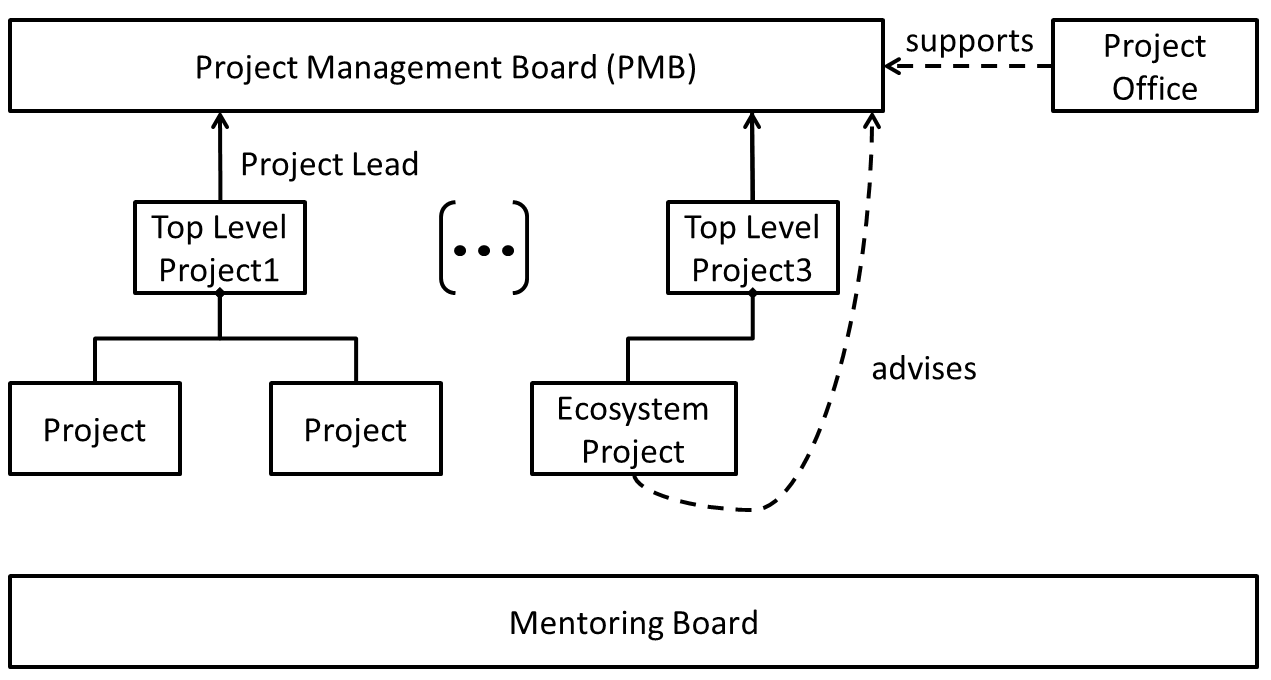
\includegraphics[width=\linewidth]{images/projectstructure.png}


Note: In the document ``\href{Process-Bootstrapping}{bootstrapping}''
the initial structure of projects, PMB and board members is described.

The descendants of a Project are the Project itself and transitive
closure of its child Projects. The top parent of a Project is the
Top-Level Project at the top of the hierarchy.

Projects are the unit entity for:

\begin{itemize}

\item
  Committers
\item
  Code
\item
  Documents
\item
  Releases
\item
  IP Records
\item
  Community Awareness
\end{itemize}

\subsection{4.1 Committers}\label{committers}

Each project has exactly one set of committers. Each Project's set of
Committers is distinct from that of any other Project, including
Sub-Projects or parent Projects. All Project Committers have equal
rights and responsibilities within the Project. Partitioning of
responsibility within a Project is managed using social convention. A
Project may, for example, divide itself into logical partitions of
functionality; it is social convention that prevents Committers from one
logical partition from doing inappropriate work in another. If
finer-grained management of committer responsibilities is required, a
project should consider partitioning (via a Restructuring Review) into
two or more Sub-Projects.

The Committers of a project have the exclusive right to elect new
Committers to their Project--no other group, including a parent Project,
can force a Project to accept a new Committer.

There is no roll-up of Committers: the set of Committers on a Project is
exactly that set of people who have been explicitly elected into that
role for the project (i.e.~being a committer on a sub-project does not
give you any automatic rights on the ``parent'' project).

In practical terms, each Project has a single group of its Committers
that provides write-access to the Project's resources. Pictorially
below, we see that a Project, in addition to the various resources and
Committers it has, can also have zero or more Sub-Projects. Each of
these Sub-Projects has its own distinct set of Committers and resources.

\subsection{4.2 Resources and Releases}\label{resources-and-releases}

Each Project owns and maintains a collection of resources.

Resources may include documents, specifications, models, requirements,
source code, a project website, space on the downloads server, access to
build resources, and other services provided by the openETCS
infrastructure. The exact infrastructure used by openETCS varies over
time and is defined outside this process document.

A project is not strictly required to make use of all the resources made
available; a project might, for example, opt to not maintain a source
code repository. Such a Project might operate as an organizational unit,
or container, for several Sub-Projects. Similarly, a Project might opt
to provide a consolidated website, build and/or download site for its
Sub-Projects (the Sub-Projects would then not require those resources
for themselves).

Each Project has a single task tracker for its open tasks, issues or bug
reports.

Any Project in the Mature Phase may make a Release. A Project in the
Incubation Phase with two Mentors may make a pre-1.0 Release. A Release
may include the code from any subset of the Project's descendants.

\subsection{4.3 Community Awareness}\label{community-awareness}

Projects are the level of communication with the larger openETCS
community and ecosystem. Projects may either have their own
communications (website, mailing lists, forums/newsgroups, etc) or they
may be part of a parent Project's communications (website, mailing list,
forums/newsgroups, etc). In either case, the Project is required to
maintain an open and public communication channel with the community
including, but not limited to, project plans, schedules, design
discussions, and so on.

All Projects must make the communication channels easy to find. Projects
are further required to make the separate communication channels of
their child Projects (if any) easy to find.

Any Project in the Incubation Phase must correctly identify its website
and Releases. A Project with at least one descendant Project in
Incubation Phase must correctly annotate its own website so as to notify
the community that incubating Projects exist in its hierarchy. Any
Release containing code from an Incubation Phase project must be
correctly labeled, i.e., the Incubation Phase is viral and expands to
cover all Releases in which it is included.

\subsection{4.4 Scope}\label{scope}

Each Top-Level Project has a Charter which describes the purpose, Scope,
and operational rules for the Top-Level Project. The Charter should
refer to, and describe any refinements to, the provisions of this
Development Process. The PMB approves the Charter of each Top-Level
Project, if it divers from this process.

Sub-Projects do not have separate Charters; Sub-Projects operate under
the Charter of their parent Top-Level Project.

All Projects have a defined Scope and all initiatives within that
Project are required to reside within that Scope. Initiatives and code
that is found to be outside the Scope of a Project may result in the
termination of the Project.

The Scope of a Sub-Project is defined by the initial project proposal as
reviewed and approved by the Project Management Board (PMB) (as further
defined below) of the Project's Project's top parent. A Project's Scope
must be a subset of its parent's Scope. \#\#\# 4.5 Leaders

There are two different types of Project leadership at openETCS: The
Project Management Board (PMB) and Project Leads. Both forms of
leadership are required to:

\begin{itemize}

\item
  ensure that their Project is operating effectively by guiding the
  overall direction and by removing obstacles, solving problems, and
  resolving conflicts;
\item
  operate using open source rules of engagement: meritocracy,
  transparency, and open participation; and ensure that the Project and
  its Sub-Projects (if any) conform to the openETCS IP Policy and
  Procedures.
\end{itemize}

The leadership for a Project is composed of the Project's Project
Lead(s), the leadership of the parent Project (if any) and the project
lead of the Top-Level Project.

\paragraph{4.5.1 Project Lead}\label{project-lead}

openETCS Projects are managed by one or more Project Leads. Project
Leads are responsible for ensuring that their Project's Committers are
following the openETCS Development Process, and that the project is
engaging in the right sorts of activities to develop vibrant communities
of users, adopters, and contributors. The initial project leadership is
appointed and approved in the creation review. Subsequently, additional
Project Leads must be elected by the project's Committers and approved
by the PMB.

In the unlikely event that a member of the Project leadership becomes
disruptive to the process or ceases to contribute for an extended
period, the member may be removed by the unanimous vote of the remaining
Project Leads (if there are at least two other Project Leads), or
unanimous vote of the PMB.

In exceptional situations, such as projects with zero active committers
or projects with disruptive Committers and no effective Project Leads,
the Project Leadership Chain has the authority to make changes (add,
remove) to the set of committers and/or Project Leads of that project.

\paragraph{4.5.2 Project Management Committee
(PMC)}\label{project-management-committee-pmc}

If top-level projects grow, the PMB can nominate a Project Management
Committee (PMC). A PMC has one or more PMC Leads and zero or more PMC
Members. Together the PMC provides oversight and overall leadership for
the projects that fall under their top-level project. The PMC as a
whole, and the PMC Leads in particular, are ultimately responsible for
ensuring that the openETCS Development Process is understood and
followed by their projects. The PMC is additionally responsible for
maintaining the top-level project's charter and aprooving new projects
and committers.

PMC members are elected by the existing PMC Leads and Members, and
approved by the PMB. \#\#\# 4.6 Committers and Contributors

Each Project has a Development Team, led by the Project Leaders. The
Development Team is composed of Committers and Contributors.
Contributors are individuals who contribute content, code, fixes, tests,
documentation, or other work that is part of the Project. Committers
have write access to the Project's resources (repository, task tracking
system, website, build server, downloads, etc.) and are expected to
influence the Project's development. See
\href{Committer-Guidelines}{these guidelines and checklists} for
electing a new committer.

Contributors who have the trust of the Project's Committers can, through
election, be promoted Committer for that Project. The breadth of a
Committer's influence corresponds to the breadth of their contribution.
A Development Team's Contributors and Committers may (and should) come
from a diverse set of organizations. A Committer gains voting rights
allowing them to affect the future of the Project. Becoming a Committer
is a privilege that is earned by contributing and showing discipline and
good judgment. It is a responsibility that should be neither given nor
taken lightly, nor is it a right based on employment by any company
employing existing committers.

The election process begins with an existing Committer on the same
Project nominating the Contributor. The Project's Committers will vote
for a period of no less than one week of standard business days. If
there are at least three (3) positive votes and no negative votes within
the voting period, the Contributor is recommended to the project's PMB
for commit privileges. If there are three (3) or fewer Committers on the
Project, a unanimous positive vote of all Committers is substituted. If
the PMB approves, and the Contributor signs the appropriate Committer
legal agreements (wherein, at the very least, the Developer agrees to
contribute under the EUPL), the Contributor becomes a Committer and is
given write access to the source code for that Project.

At times, Committers may become inactive for a variety of reasons. The
decision making process of the Project relies on active committers who
respond to discussions and vote in a constructive and timely manner. The
Project Leaders are responsible for ensuring the smooth operation of the
Project. A Committer who is disruptive, does not participate actively,
or has been inactive for an extended period may have his or her commit
status revoked by the Project Leaders. (Unless otherwise specified, ``an
extended period'' is defined as ``no activity for more than six
months''.)

Active participation in the appropriate developer mailing lists is a
responsibility of all Committers, and is critical to the success of the
Project. Committers are required to monitor and contribute to the
mailinglists.

Committers are required to monitor the mailing lists associated with the
Project. This is a condition of being granted commit rights to the
Project. It is mandatory because committers must participate in votes
(which in some cases require a certain minimum number of votes) and must
respond to the mailing list in a timely fashion in order to facilitate
the smooth operation of the Project. When a Committer is granted commit
rights they will be added to the appropriate mailing lists. A Committer
must not be unsubscribed from a developer mailing list unless their
associated commit privileges are also revoked.

Committers are required to track, participate in, and vote on, relevant
discussions in their associated Projects and components. There are three
voting responses: +1 (yes), -1 (no, or veto), and 0 (abstain).

Committers are responsible for proactively reporting problems in the
task tracking system, and annotating problem reports with status
information, explanations, clarifications, or requests for more
information from the submitter. Committers are responsible for updating
problem reports when they have done work related to the problem.

Committer, PMC Lead, Project Lead, and Board Representative(s) are
roles; an individual may take on more than one of these roles
simultaneously.

\subsection{4.8 Project Management Board
(PMB)}\label{project-management-board-pmb}

The PMB is responsible for (i) maintaining and revising the openETCS
Development Process, (ii) asure the implementation of the requirements
of the development process described in this document.(iii) monitoring,
guiding, and influencing the software architectures used by Projects,
(iv) establishing the communication between specification projects and
implementation projects

\subsection{4.9 Mentoring Board}\label{mentoring-board}

The Mentoring board is responsible for mentoring projects and advising.

\subsection{4.10 Project Office}\label{project-office}

The project office is responsible for administrative tasks around the
openETCS development process. Therefore the project office has the
ability to grant access rights to projects, can maintain the openETCS
documentation and so on. The project office is instructed to clarify,
expand, and extend this Process by creating a set of openECTS Project
Development Guidelines. The project office is not permitted to override
or ignore the requirements listed in this document without agreement of
the PMB.

\subsection{4.11 Ecosystem Project}\label{ecosystem-project}

The ecosystem is a regular project, which is responsible for developing
proposes solutions for the infrastructure as well as process refinements
and additional guidelines. Therefore the ecosystem collaborates with the
project office.

\subsection{4.12 Incubator Projects}\label{incubator-projects}

A Project may designate a Sub-Project as an ``Incubator''. An Incubator
is a Project that is intended to perpetually remain in the Incubation
phase. Incubators are an excellent place to innovate, test new ideas,
grow functionality that may one day be moved into another Project, and
develop new committers.

Incubator Projects never have releases; they do not require yearly
continuation reviews. Incubators may have builds, and downloads. They
conform to the standard incubation branding requirements and are subject
to the IP due diligence rules outlined for incubating Projects.
Incubators do not graduate.

The scope of an Incubator Project must fall within the scope of its
parent project. The committer group of the Incubator Project must
overlap with that of the parent project (at least one committer from the
parent project must be a committer for the Incubator). Incubator
projects do not require mentors (the parent project's committers are
responsible for ensuring that the Incubator project conform to the rules
set forth by the openETCS Development Process).

An Incubator project should designated as such by including the word
``Incubator'' in its name (e.g. ``VV Incubator''). To do otherwise is
considered exceptional and requires approval from the PMB.

Only Top-Level Projects and Projects in the Mature phase may create an
Incubator. Incubators are created via a Creation Review. Alternatively,
an Incubator can be created as part of a Graduation, Promotion, or
Restructuring Review. A proposal is not required to create an Incubator
project.

\section{5. Development Process}\label{development-process}

Projects must work within their Scope. Projects that desire to expand
beyond their current Scope must seek an enlargement of their Scope using
a public Review as described below. Further, projects must fit within
the scope defined by their containing projects and the scope defined in
the charter of their Top-Level Project.

All projects are required to report their status at least quarterly
using the defined status reporting procedures.

Projects must provide advanced notification of upcoming features and
frameworks via their Project Plan. \#\#\# 6.1 Mentors

New Proposals that intend to do a Release are required to have at least
two Mentors. New Proposals that will only release as part of a parent
Project's Release are not required to have Mentors. Mentors must be
members of the Mentoring Board. The Mentors (including name,
affiliation, and current projects/roles) must be listed in the Proposal.
Mentors are required to monitor and advise the new Project during its
Incubation Phase, but are released from that duty once the Project
graduates to the Mature Phase.

\subsection{6.2 Project Lifecycle}\label{project-lifecycle}

Projects go through six distinct phases. The transitions from phase to
phase are open and transparent public reviews.

{[}{[}/images/Development-process-small.gif{]}{]}

\paragraph{6.2.1 Pre-proposal}\label{pre-proposal}

See \href{Project-Proposal-Guidelines}{guidelines and checklists} about
writing a proposal.

An individual or group of individuals declares their interest in, and
rationale for, establishing a project. The menotring board will assist
such groups in the preparation of a project Proposal. The Pre-proposal
phase ends when the Proposal is published by the project office and
announced to the membership by the project office.

\paragraph{6.2.2 Proposal}\label{proposal}

See \href{Project-Proposal-Guidelines}{guidelines and checklists} about
gathering support for a proposal.

The proposers, in conjunction with the destination PMB and the
community, collaborate in public to enhance, refine, and clarify the
proposal. Mentors (if necessary) for the project must be identified
during this phase.

\begin{itemize}

\item
  The Proposal phase ends with a Creation Review, or withdrawal.
\item
  The Proposal may be withdrawn by the proposers.
\item
  The project office will withdraw a proposal that has been inactive for
  more than six months.
\end{itemize}

\paragraph{6.2.3 Incubation}\label{incubation}

See guidelines and checklists about incubation.

After the project has been created, the purpose of the incubation phase
is to establish a fully-functioning open-source project. In this
context, incubation is about developing the process, the community, and
the technology. Incubation is a phase rather than a place: new projects
may be incubated under any existing Project.

\begin{itemize}

\item
  The Incubation phase may continue with a Continuation Review or a
  Release Review.
\item
  Top-Level Projects cannot be incubated and can only be created from
  one or more existing Mature-phase Projects.
\item
  The Incubation phase ends with a Graduation Review or a Termination
  Review.
\item
  Designated Incubator Projects may remain perpetually in the Incubation
  phase; no reviews are required.
\end{itemize}

Many Projects are proposed and initiated by individuals with extensive
and successful software development experience. This document attempts
to define a process that is sufficiently flexible to learn from all its
participants. At the same time, however, the Incubation phase is useful
for new Projects to learn the community-defined open source processes.
See guidelines and checklists for utilizing the Parallel IP process.

Only projects that are properly identified as being in the incubation
phase (including designated Incubator Projects) may use the Parallel IP
process to reduce IP clearance process for new contributions. \#\#\#\#
6.2.4 Mature See guidelines and checklists about the mature phase.

The project team has demonstrated that they are an open-source project
with an open and transparent process; an actively involved and growing
community; and Quality work products. The project is now a mature member
of the openETCS Community. Major releases continue to go through Release
Reviews.

\begin{itemize}

\item
  Mature phase projects have Releases through Release Reviews.
\item
  A Mature Project may be promoted to a Top-Level Project through a
  Promotion Review.
\item
  A Mature Project that does not participate in a Release in given year
  may continue through a Continuation Review.
\item
  Inactive Mature phase projects may be archived through a Termination
  Review.
\end{itemize}

\paragraph{6.2.5 Top-Level}\label{top-level}

See guidelines and checklists about being a top-level project.

Projects that have demonstrated the characteristics of a Top-Level
Project (e.g., consistent leadership in a technical area and the
recruitment of a wider developer community) can be promoted to Top-Level
Project status. This promotion occurs through a Promotion Review.
\#\#\#\# 6.2.6 Archived See guidelines and checklists for archiving
projects.

Projects that become inactive, either through dwindling resources or by
reaching their natural conclusion, are archived. Projects can reach
their natural conclusion in a number of ways: for example, a project
might become so popular that it is absorbed into one of the other major
frameworks. Projects are moved to Archived status through a Termination
Review.

If there is sufficient community interest in reactivating an Archived
Project, the Project will start again with Creation Review. As there
must be good reasons to have moved a Project to the Archives, the
Creation Review provides a sufficiently high bar to prove that those
reasons are no longer valid. \#\# 6.3 Reviews

The openETCS Development Process is predicated on open and transparent
behavior. All major changes to projects must be announced and reviewed
by the membership-at-large. Major changes include the Project Phase
transitions as well as the introduction or exclusion of significant new
technology or capability. It is a clear requirement of this document
that members who are monitoring the appropriate media channels (e.g.,
mailing lists or RSS feeds) not be surprised by the post-facto actions
of the Projects.

All Projects are required to participate in at least one Review per
year.

For each Review, the project leadership prepares documentation for, and
receives feedback from, the community.

A Review is a fairly comprehensive process. Gathering the material for a
Review and preparing the documentation is a non-trivial effort, but the
introspection offered by this exercise is useful for the Project and
results are very useful for the entire community. In addition, Reviews
have a specific relationship to the requirements of the IP Policy.

All Reviews have the same general process:

\begin{itemize}

\item
  Projects are responsible for initiating the appropriate reviews.
  However, if a Project does not do so and the project office believes a
  Review is necessary, the project may initiate a Review on the
  Project's behalf.
\item
  A Review then continues with the Project's Leadership requesting that
  the project office schedule the Review. Prior to the start of the
  review period, the Project leadership provides the project office with
  review documentation.
\item
  The review documentation material always includes a document that
  describes the review. The minimum contents of the document are
  specified by the individual Review types.
\item
  The review documentation must be available in a format that anyone in
  the openETCS membership can review. PDF and HTML are acceptable single
  formats.
\item
  The review documentation must have a correct copyright statement and
  license.
\item
  The review documentation must be archival quality. This means that the
  materials must be comprehensible and complete on their own without
  requiring explanation by a human presenter, reference to a wiki, or to
  other non-archived web pages.
\item
  The project office announces the Review schedule and makes the
  documentation available to the membership-at-large.
\end{itemize}

The criteria for the successful completion of each type of Review will
be documented in writing by the project office in guidelines made
available via the openETCS website. Such guidelines will include, but
are not limited to the following:

\begin{itemize}

\item
  Clear evidence that the project has vibrant committer, adopter and
  user communities as appropriate for the type of Review.
\item
  Reasonable diversity in its committer population as appropriate for
  the type of Review. Diversity status must be provided not only as
  number of people/companies, but also in terms of effort provided by
  those people/companies.
\item
  Documented completion of all required due diligence under the openETCS
  IP Policy.
\item
  For Continuation, Graduation and Release Reviews, the project must
  have a current project plan, in the format specified by project
  office, available to the community.
\item
  Balanced progress in creating both frameworks and extensible,
  exemplary tools.
\item
  Showcase the project's quality through project-team chosen metrics and
  measures, e.g., coupling, cyclomatic complexity, test/code coverage,
  documentation of extensions points, etc.
\end{itemize}

The Review period is open for no less than one week and usually no more
than two weeks of generally accepted business days.

The Review begins with the project offices's posting of the review
materials at the start of the Review period. The proper functioning of
the openETCS Development Process is contingent on the active
participation of the openETCS Members and Committers, especially in
Reviews, thus each Review has an project-designated discussion and
feedback communication channel: a forum/newgroup, a mailing list, or
some other public forum. * If a Committer election is required for a
Review (for example, for a Creation Review), then it is held
simultaneously with the Review period. Thus the election and the Review
will end at the same time, allowing quick and efficient provisioning of
the resulting Project. * The project office approves or fails the Review
based on the public comments, the scope of the Project, and the Purposes
of the openETCS project. * The Review ends with the announcement of the
results in the defined Review communication channel (the project office
will request that the Project Lead make this announcement).

If any Member believes that the project office has acted incorrectly in
approving or failing a Review may appeal to the PMB to review the
decision. \#\#\# 6.3.1 Creation Review See guidelines and checklists
about Creation Reviews.

The purpose of the Creation Review is to assess the community and
membership response to the proposal, to verify that appropriate
resources are available for the project to achieve its plan, and to
serve as a committer election for the project's initial Committers. The
openETCS strives not to be a repository of ``code dumps'' and thus
projects must be sufficiently staffed for forward progress.

The Creation Review documents must include short nomination bios of the
proposed initial committers. These bios should discuss their
relationship to, and history with, the incoming code and/or their
involvement with the area/technologies covered by the proposal. The goal
is to help keep any legacy contributors connected to new project and
explain that connection to the current and future openETCS project, as
well as justify the initial Committers' participation in a meritocracy.
\#\#\# 6.3.2 Graduation Review See guidelines and checklists about
Graduation Reviews.

The purpose of the Graduation Review is to confirm that the Project
is/has:

\begin{itemize}

\item
  a working and demonstrable code base of sufficiently high quality
\item
  active and sufficiently diverse communities appropriate to the size of
  the graduating code base: adopters, developers, and users
\item
  operating fully in the open following the Principles and Purposes of
  openETCS
\item
  a credit to openETCS and is functioning well within the larger
  openETCS community
\end{itemize}

The Graduation Review is about the phase change from Incubation Phase to
Mature Phase. If the Project and/or some of its code is simultaneously
relocating to another Project, the Graduation Review will be combined
with a Restructuring Review. \#\#\# 6.3.3 Release Review See guidelines
and checklists about Release Reviews.

The purposes of a Release Review are: to summarize the accomplishments
of the release, to verify that the IP Policy has been followed and all
approvals have been received, to highlight any remaining quality and/or
architectural issues, and to verify that the project is continuing to
operate according to the Principles and Purposes of openETCS . 6.3.4
Promotion Review

The purpose of a Promotion Review is to determine if the Project has
demonstrated the characteristics of a Top-Level Project, e.g.,
consistent leadership in a technical area and the recruitment of a wider
developer community. The Project will already be a well-functioning
Mature openETCS Project, so evidence to the contrary will be a negative
for promotion. Top-Level Projects, both through their existence and
their Council memberships, have substantial influence over direction and
operation of openETCS, thus it behooves the membership to grant
Top-Level status only for merit: for demonstrated service to the larger
openETCS ecosystem. \#\#\# 6.3.5 Continuation Review

The purpose of a Continuation Review is to verify that a Proposal or
Project continues to be a viable effort and a credit to openETCS. The
Project team will be expected to explain the recent technical progress
and to demonstrate sufficient adopter, developer, and user support for
the Project. The goal of the Continuation Review is to avoid having
inactive projects looking promising but never actually delivering
extensible frameworks and exemplary tools to the ecosystem. \#\#\# 6.3.6
Termination Review See Termination Review ``How To'' for more
information.

The purpose of a Termination Review is to provide a final opportunity
for the Committers and/or openETCS community to discuss the proposed
withdrawal of a Proposal or archiving of a Project. The desired outcome
is to find sufficient evidence of renewed interest and resources in
keeping the Project or Proposal active. \#\#\# 6.3.7 Move Review

A Move Review is considered to be a special type of Restructuring
Review. \#\#\# 6.3.8 Restructuring Review

The purpose of a Restructuring Review is to notify the community of your
intent to make significant changes to one or more projects.
``Significant changes'' includes:

\begin{itemize}

\item
  Movement of significant chunks of functionality from one project to
  another;
\item
  Modification of the project structure, e.g.~combining multiple
  projects into a single project, or decomposing a single project into
  multiple projects; and/or
\item
  Change of project scope.
\end{itemize}

A Restructuring Review may include the movement of significant chunks of
code. A move is considered significant if it has an impact on the
community (i.e.~if segments of the community will notice that the code
has moved). This may include entire projects, bundles, and features, but
likely excludes small fragments, code snippets and individual files. The
IP Log of all moved code must be reviewed prior to the start of the
review period (this, typically, is a subset of the project's IP Log). If
all of the code is moved out of a project, a Termination Review for that
project can be combined with the Restructuring Review.

Note that, regardless of whether or not a review is required, moving
code from one Project to another is subject to the IP Policy.

A Restructuring Review may necessitate the construction of one or more
new projects. This tends to occur when an existing project is decomposed
into two or more projects. In this case, a Restructuring Review is
similar to a Creation Review. Any new projects that are created as part
of a Restructuring Review must have their scope explicitly specified as
part of the review. The scope of any new project must be a subset of the
scope of the original project. Likewise, the set of committers assigned
to a new project must be a subset of the committers of the original
project (additional committers can be elected to the new project after
it is created). Any new projects that fall outside of the scope of the
original project, or wish to establish a different set of committers,
must undergo the full project creation process.

Committers can be moved along with code into a new project as part of
the project provisioning process. Committers cannot be moved along with
code into an existing project. In this case, the existing project must
elect the new committers into the project.

A project is expected to socialize pending changes using established
communication channels prior to initiating the review. A Restructuring
Review must provide the community with at least one week to review and
respond to the changes. Prior to the start of that review period, the
community must be provided with (via the project office) completed
review documentation that describes in specific terms what will be
changed as part of the restructuring.

This may include: * Name, description, scope, and committer lists of new
projects that need to be created; * Source and target locations for
moves of source code directories; * Reorganization of builds and
downloads; * Contribution questionnaires (CQs) that need to be moved or
piggy-back CQs that must be created; * Location of the approved IP Log;
and * Other information that helps the community understand the change.

\subsection{6.3.9 Combining Reviews}\label{combining-reviews}

Reviews can be combined at the discretion of the PMB and project office.
Multiple Projects may participate in a single Review. Similarly,
multiple review types can be engaged in simultaneously. A parent Project
may, for example, engage in an aggregated Release Review involving
itself and some or all of its child projects; a consolidated
Restructuring Review may move the code for several projects; or a
Release Review may be combined with a Graduation Review. When multiple
reviews are combined, the review documentation must explicitly state all
of the Projects and types of reviews involved, and include the required
information about each.

It should be noted that the purpose of combining reviews is to better
serve the community, rather than to reduce effort on the part of the
project (though it is fortunate when it does both). Combining a Release
and Graduation review, or aggregating a Release Review of a Project and
several of it's child Projects generally makes sense. Combining Release
Reviews for multiple unrelated projects most likely does not. \#\# 6.4
Releases

(Most of this section is borrowed and paraphrased from the excellent
Apache Software Foundation Releases FAQ. The openETCS community has many
of the same beliefs about Releases as does the Apache community and
their words were already excellent. The Apache Software Foundation
Releases FAQ is distributed under the Apache License, Version 2.0.)

Releases are, by definition, anything that is distributed outside of the
Committers of a Project. If users are being directed to download a
build, then that build has been released (modulo the exceptions below).
All Projects and Committers must obey the openETCS requirements on
approving any release.

(Exception 1: nightly and integration builds) During the process of
developing software and preparing a Release, various nightly and
integration builds are made available to the developer community for
testing purposes. Do not include any links on the project website,
blogs, wikis, etc. that might encourage non-early-adopters to download
and use nightly builds, release candidates, or any other similar package
(links aimed at early-adopters and the project's developers are both
permitted and encouraged). The only people who are supposed to know
about such packages are the people following the developer mailing list
and thus are aware of the limitations of such builds.

(Exception 2: milestone and release candidate builds) Projects are
encouraged to use an agile development process including regular
milestones (for example, six week milestones). Milestones and release
candidates are ``almost releases'' intended for adoption and testing by
early adopters. Projects are allowed to have links on the project
website, blogs, wikis, etc. to encourage these
outside-the-committer-circle early adopters to download and test the
milestones and release candidates, but such communications must include
caveats explaining that these are not official Releases.

\begin{itemize}

\item
  Milestones are to be labeled x.yMz, e.g., 2.3M1 (milestone 1 towards
  version 2.3), 2.3M2 (milestone 2 towards version 2.3), etc.
\item
  Release candidates are to be labeled x.yRCz, e.g., 2.3RC1 (release
  candidate 1 towards version 2.3).
\item
  Official Releases are the only downloads allowed to be labeled with
  x.y, e.g., 0.5, 1.0, 2.3, etc.
\end{itemize}

All official Releases must have a successful Release Review before being
made available for download.

(Exception 3: bug fix releases with no new features) Bug fix releases
(x.y.z, e.g., 2.3.1) with no new features over the base release (e.g.,
2.3) are allowed to be released without an additional Release Review. If
a bug fix release contains new features, then the Project must have a
full Release Review.

Under no circumstances are builds and milestones to be used as a
substitute for doing proper official Releases. Proper Release management
and reviews is a key aspect of openETCS Quality.


\section{6.5 Grievance Handling}

When a Member has a concern about a Project, the Member will raise that
concern with the Project's Leadership. If the Member is not satisfied
with the result, the Member can raise the concern with the parent
Project's Leadership. The Member can continue appeals up the Project
Leadership Chain and, if still not satisfied, thence to the project
office and finally to the Mentoring Board. All appeals and discussions
will abide by the Guiding Principles of being open, transparent, and
public.

Member concerns may include:

\begin{itemize}

\item
  Out of Scope. It is alleged that a Project is exceeding its approved
  scope.
\item
  Dysfunctional. It is alleged that a Project is not functioning
  correctly or is in violation of one or more requirements of the
  Development Process.
\item
  Contributor Appeal. It is alleged that a Contributor who desires to be
  a Committer is not being treated fairly.
\item
  Invalid Veto. It is alleged that a -1 vote on a Review is not in the
  interests of the Project and/or of openETCS.
\end{itemize}

A variety of grievance resolutions are available to the project office
up to, and including, rebooting or restarting a project with new
Committers and leadership.

